\section{Analisi}


\begin{frame}
    \frametitle{Variazioni frontali}
    \framesubtitle{}

    \begin{figure}
        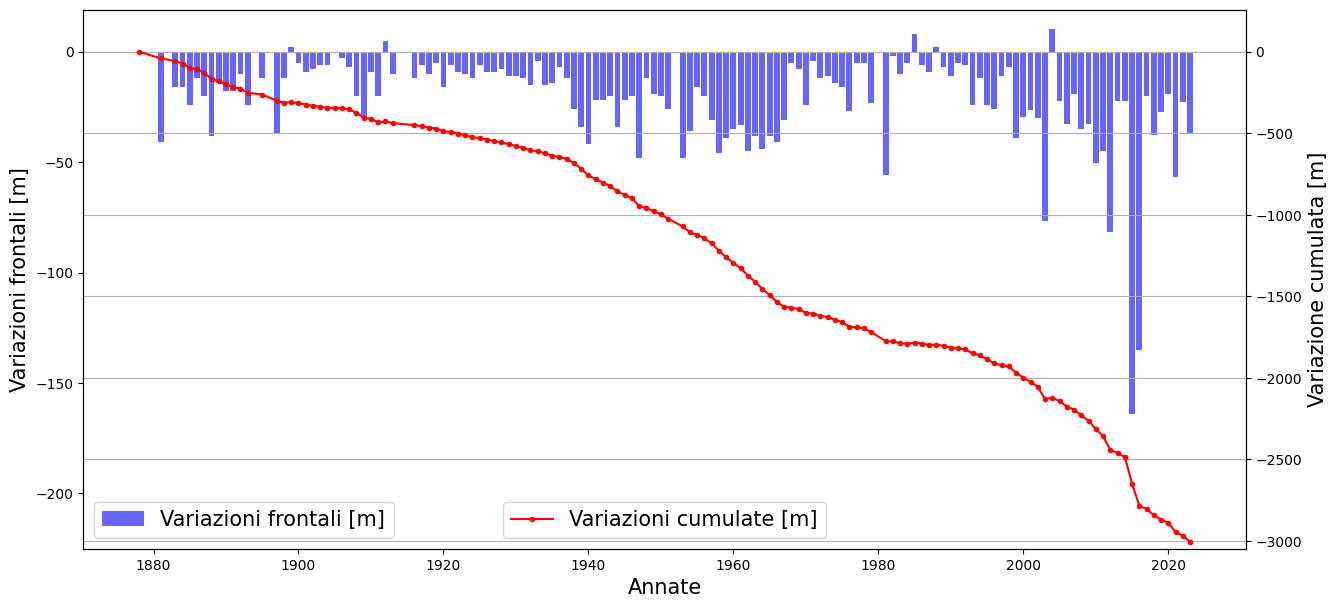
\includegraphics[width=0.9\textwidth]{Immagini/variazioniSovrapposte.png}
        \caption{Dati da \cite{GLAMOS23}}
    \end{figure}
  
\end{frame}


\begin{frame}
    \frametitle{Ablation stakes Morteratsch}
    \framesubtitle{}

    \begin{figure}
        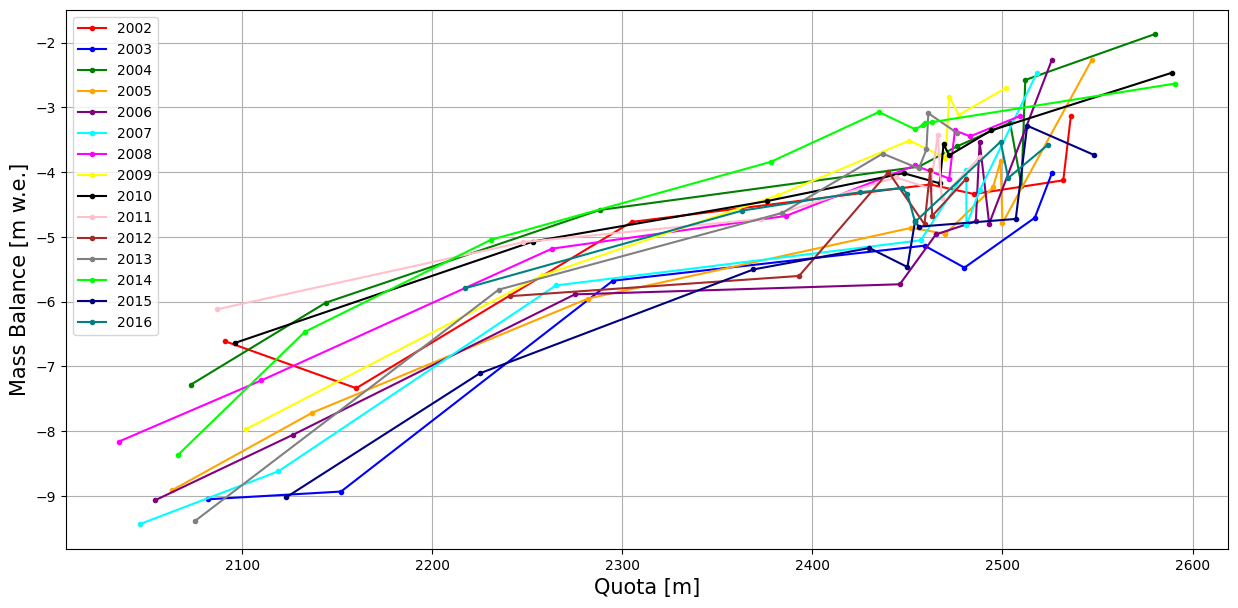
\includegraphics[width=0.9\textwidth]{Immagini/annateMassBalanceMorteratsch.png}
        \caption{Dati da \cite{STAT2018}}
    \end{figure}
  
\end{frame}


\begin{frame}
    \frametitle{Ablation stakes Vadret Pers}
    \framesubtitle{}

    \begin{figure}
        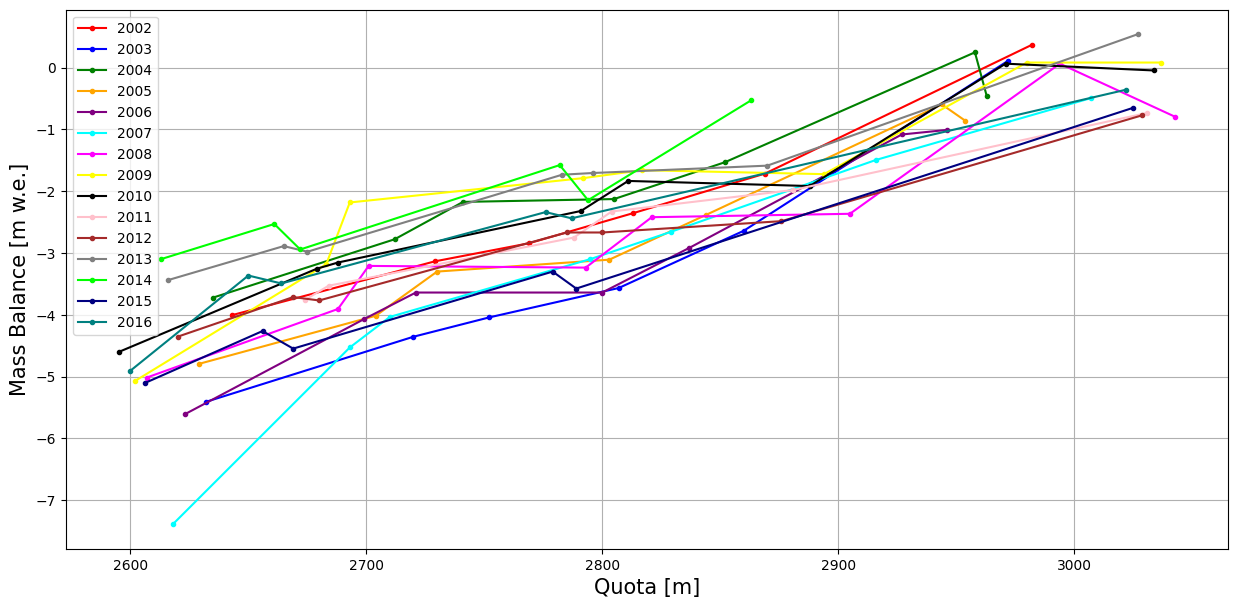
\includegraphics[width=0.9\textwidth]{Immagini/annateMassBalanceVadretPers.png}
        \caption{Dati da \cite{STAT2018}}
    \end{figure}
  
\end{frame}


\begin{frame}
    \frametitle{ELA Vadret Pers}
    \framesubtitle{}

    \begin{figure}
        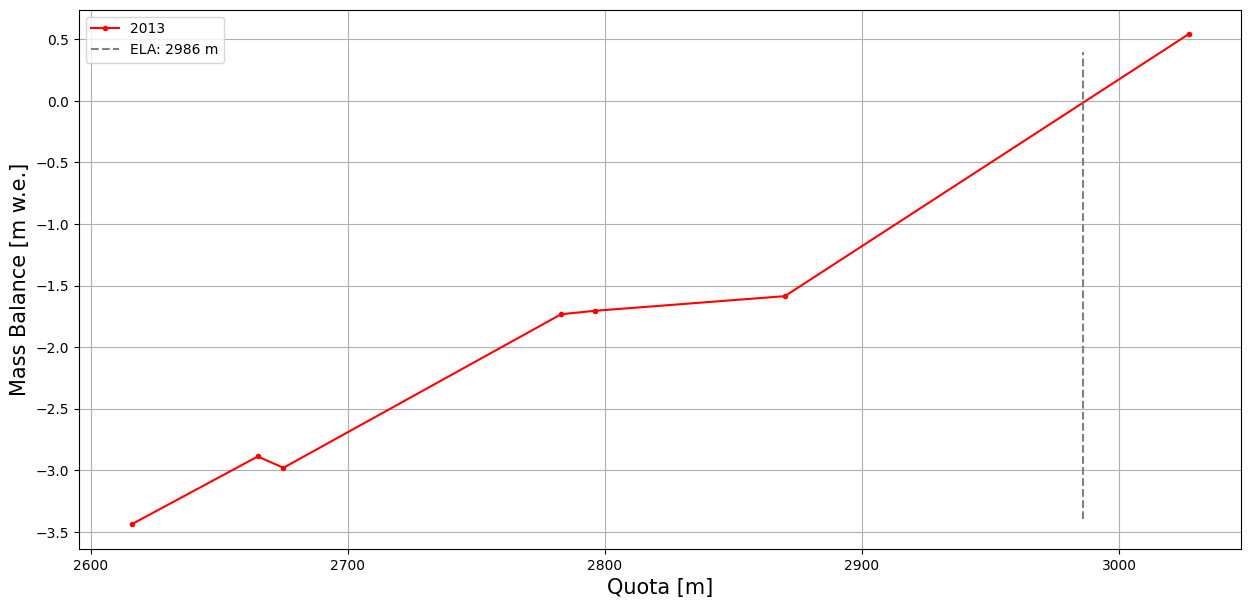
\includegraphics[width=0.9\textwidth]{Immagini/elaPers.png}
        \caption{Dati da \cite{STAT2018}}
    \end{figure}
  
\end{frame}


\begin{frame}
    \frametitle{AWS Morteratsch}
    \framesubtitle{}

    \begin{figure}
        \includegraphics[width=0.55\textwidth]{Immagini/awsMorteratsch2018.png}
        \caption{Foto da \href{https://www.projects.science.uu.nl/iceclimate/aws/alpine.php}{\textcolor{blue}{IMAU}}}
    \end{figure}
  
\end{frame}


\begin{frame}
    \frametitle{Shortwave radiation}
    \framesubtitle{}

    \begin{figure}
        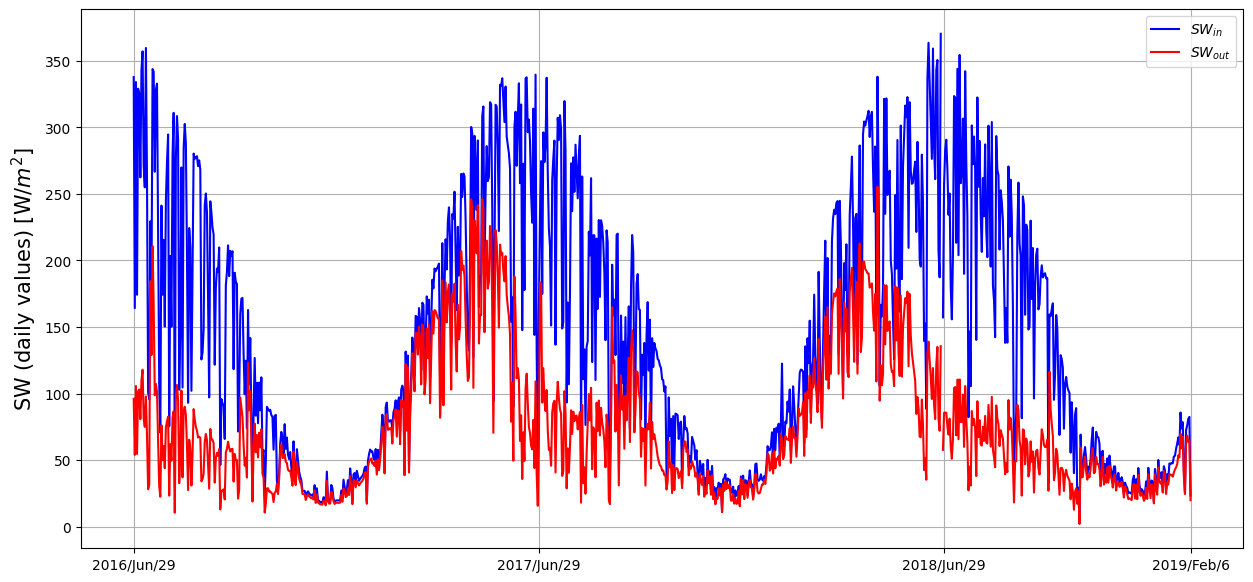
\includegraphics[width=0.9\textwidth]{Immagini/shortWaveDaily.png}
        \caption{Dati da Oerlemans}
    \end{figure}
  
\end{frame}


\begin{frame}
    \frametitle{Albedo}
    \framesubtitle

    \center
    \begin{minipage}{0.5\textwidth}
        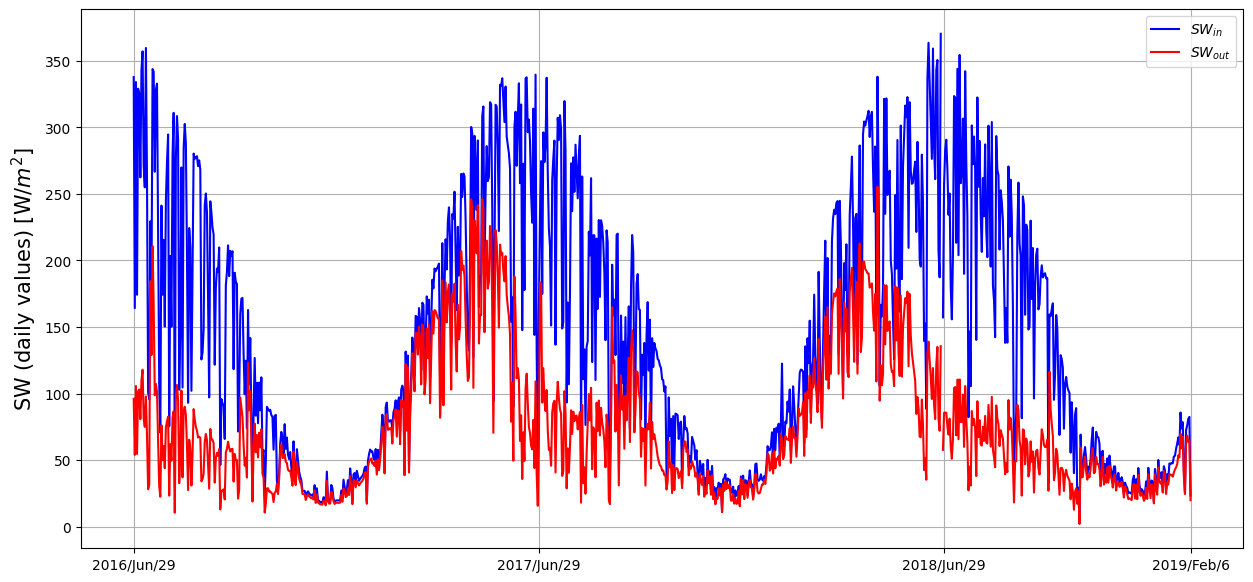
\includegraphics[width=\textwidth]{Immagini/shortWaveDaily.png}
    \end{minipage}
    \begin{minipage}{0.5\textwidth}
        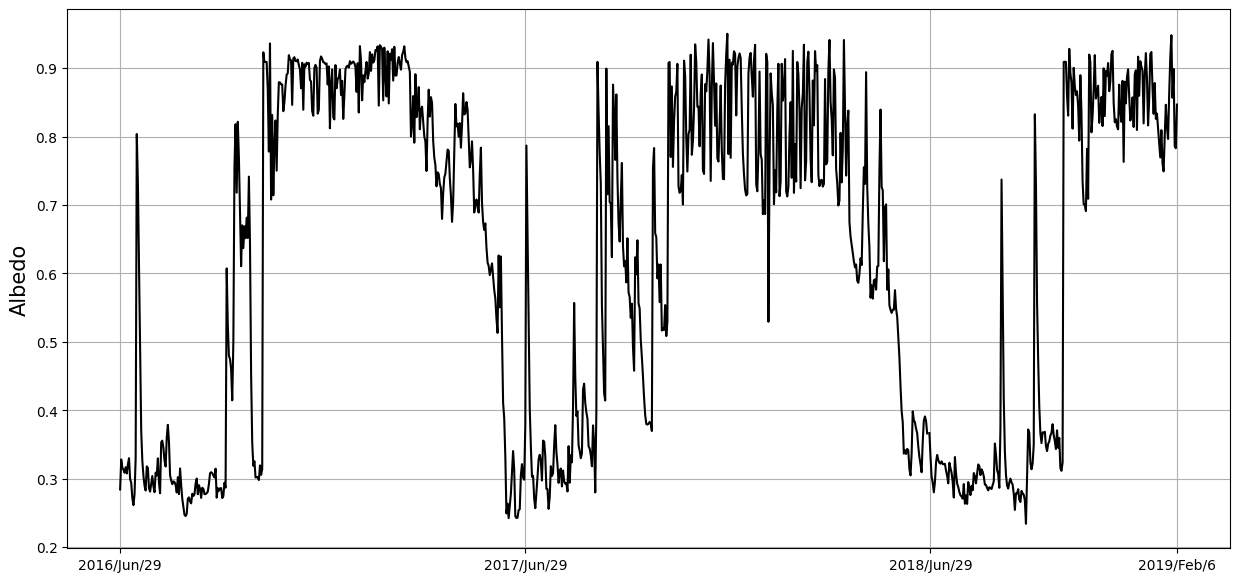
\includegraphics[width=\textwidth]{Immagini/albedoYear.png}
    \end{minipage}

\end{frame}

\begin{frame}
    \frametitle{Albedo per year}
    \framesubtitle

    \center
    \begin{figure}
        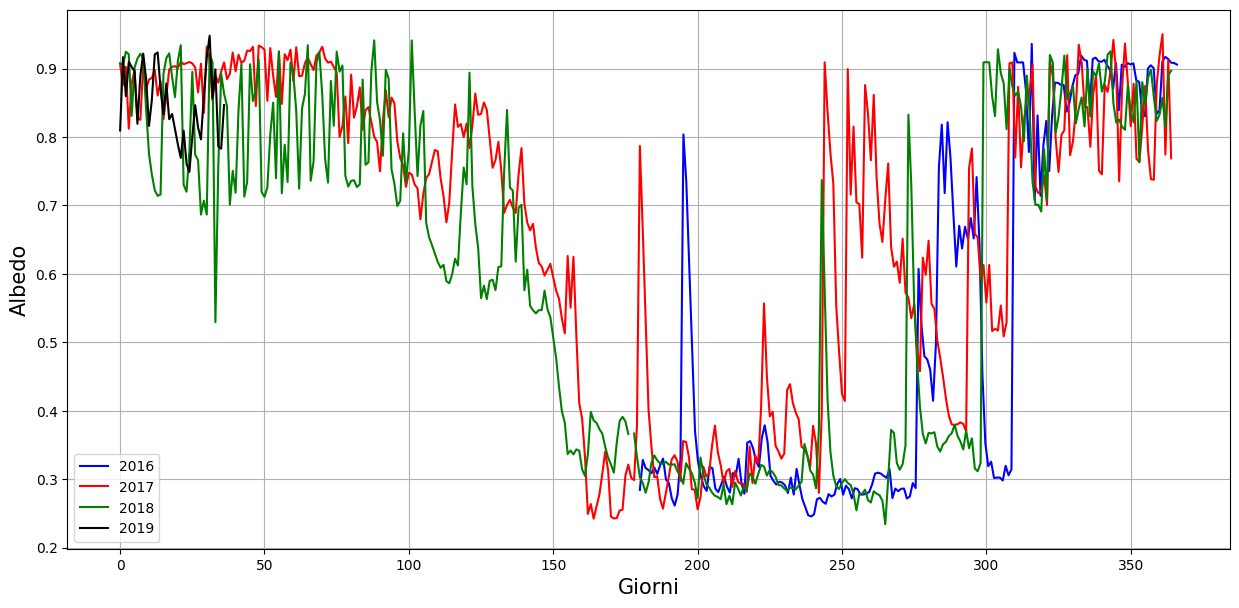
\includegraphics[width=0.9\textwidth]{Immagini/albedoPerYear.png}
        \caption{Dati da Oerlemans}
    \end{figure}

\end{frame}


\begin{frame}
    \frametitle{Longwave radiation}
    \framesubtitle{}

    \begin{figure}
        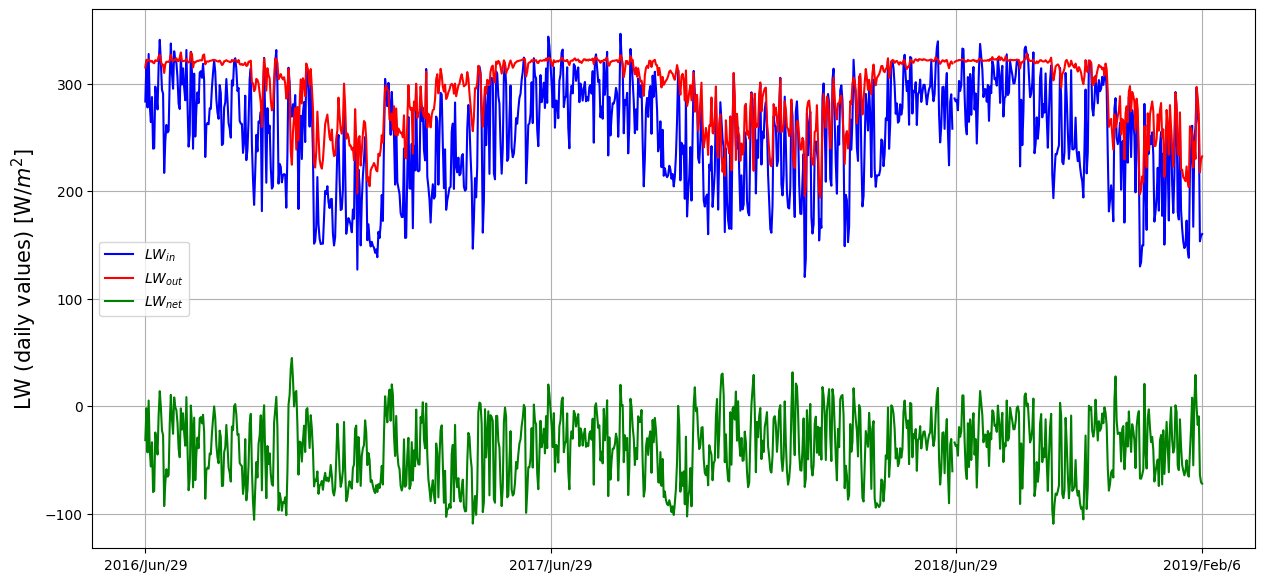
\includegraphics[width=0.9\textwidth]{Immagini/longWaveDaily.png}
        \caption{Dati da Oerlemans}
    \end{figure}
  
\end{frame}


\begin{frame}
    \frametitle{Total energy budget}
    \framesubtitle{}

    \begin{figure}
        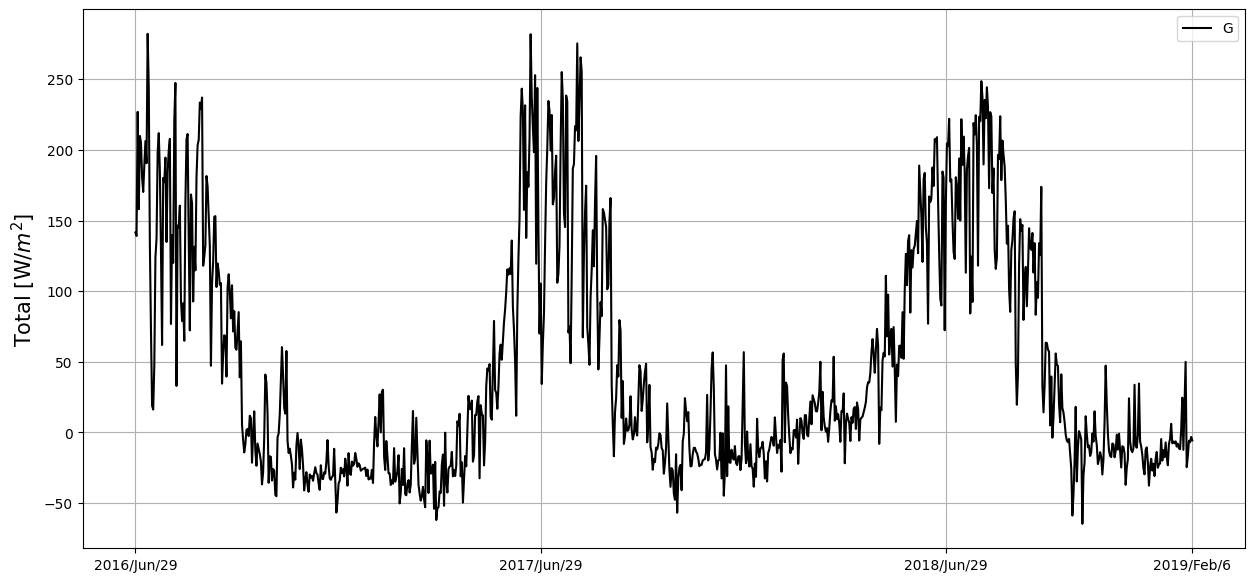
\includegraphics[width=0.9\textwidth]{Immagini/totalEnergy.png}
        \caption{Dati da Oerlemans}
    \end{figure}
  
\end{frame}


\begin{frame}
    \frametitle{Benchmark}
    \framesubtitle{}

    \begin{columns}
        
        \begin{column}{0.5\textwidth}
            \begin{figure}
                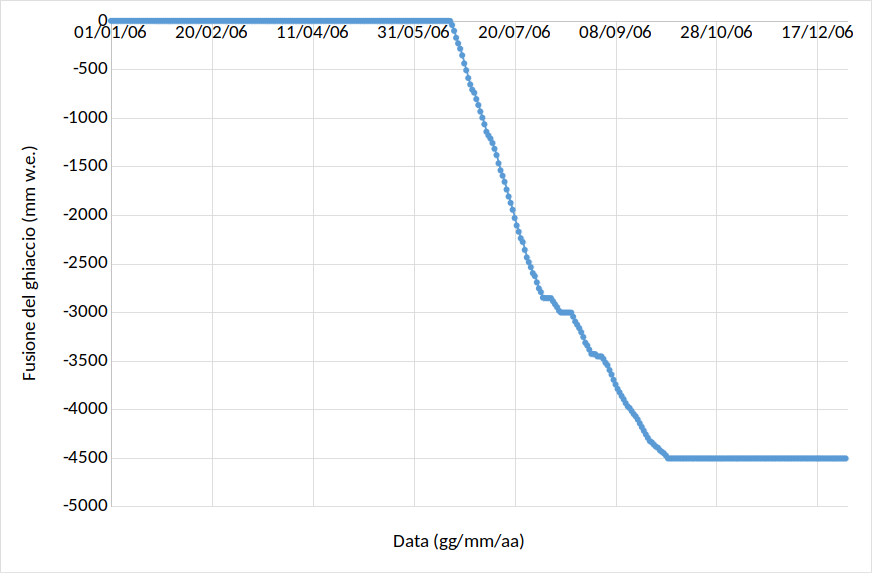
\includegraphics[width=\textwidth]{Immagini/forniLez.png}
            \end{figure}
        \end{column}
        
        \begin{column}{0.5\textwidth}
            \begin{figure}
                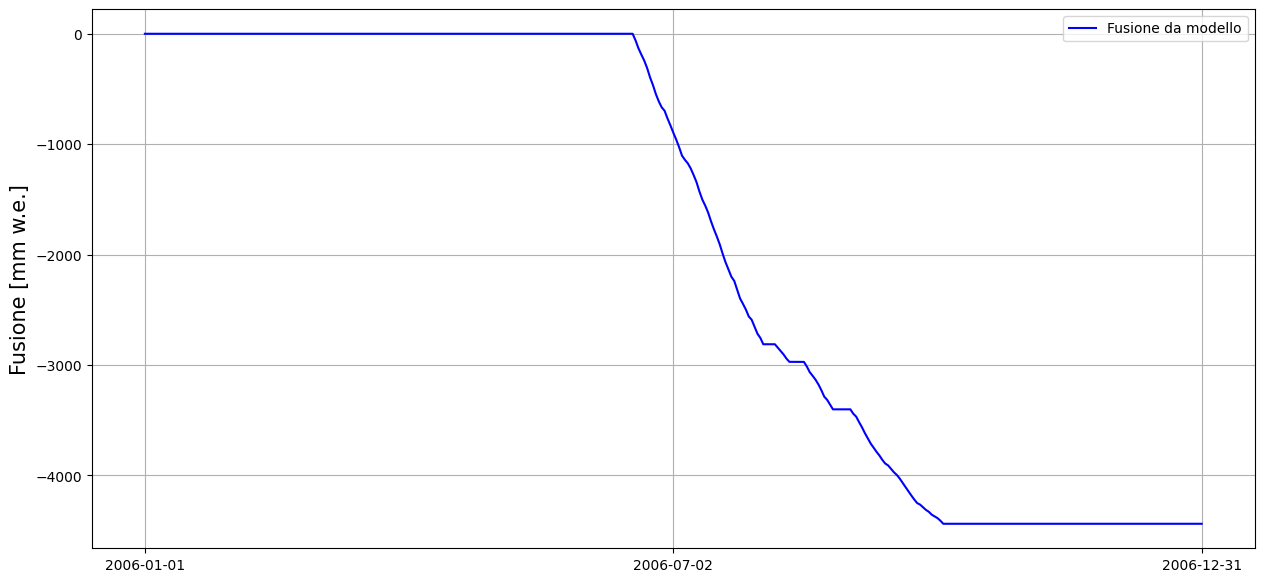
\includegraphics[width=\textwidth]{Immagini/forniBen.png}
            \end{figure}
        \end{column}
      \end{columns}
  
\end{frame}


\begin{frame}
    \frametitle{Melt}
    \framesubtitle{}

    \begin{figure}
        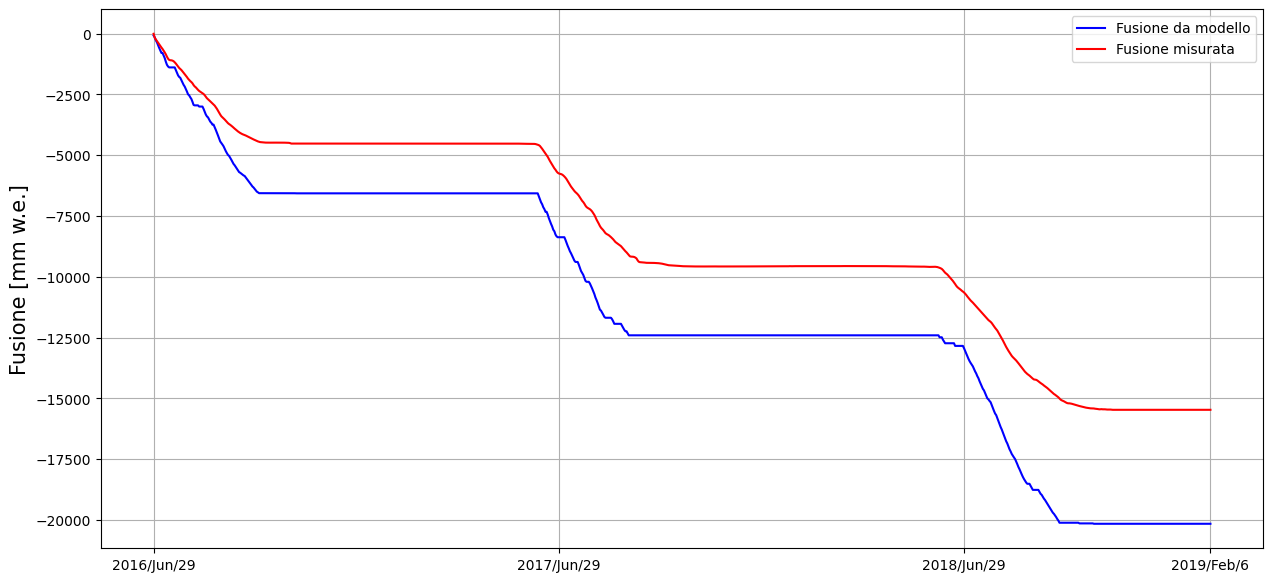
\includegraphics[width=0.9\textwidth]{Immagini/confrontoMelt.png}
        \caption{Dati da Oerlemans}
    \end{figure}
  
\end{frame}
